\documentclass{beamer}
\usetheme{Madrid}
\usefonttheme{structuresmallcapsserif}
\usefonttheme[onlymath]{serif}
%\usecolortheme{whale}
\usepackage[utf8]{inputenc}
\usepackage[spanish]{babel}
\usepackage{amsmath}
\usepackage{amsfonts}
\usepackage{amssymb}
\usepackage{mathtools}
\usepackage{graphicx}
%\usepackage{cleveref}
%\usepackage{autonum}
\usepackage{listings}
\usepackage{braket}
\usepackage{tikz}
\usepackage{bm}
\usepackage{multicol}
\usepackage{breqn}
\usepackage{physics}

\usetikzlibrary{babel}

\setbeamertemplate{caption}[numbered]

\newcommand{\V}[1]{\mathbf{#1}}
\newcommand{\Ej}{\textbf{Ejemplo: }}

\theoremstyle{example}
\newtheorem{ejemplo}{Ejemplo}[section]

\theoremstyle{example}
\newtheorem*{notacion}{Notación}

\setbeamertemplate{theorems}[numbered]
\setbeamertemplate{definitions}[numbered]

\AtBeginSection[]{
  \begin{frame}
  \vfill
  \centering
  \begin{beamercolorbox}[center,shadow=true,rounded=true]{title}
    \usebeamerfont{title}\insertsectionhead\par%
  \end{beamercolorbox}
  \vfill
  \end{frame}}

%\setbeamertemplate{section in toc}[sections numbered]
%\setbeamertemplate{subsection in toc}[subsections numbered]

\title[Decaimiento del FV en la MC]{Decaimiento del falso vacío en la Mecánica Cuántica}
%\subtitle{Física I - CAE (2020)}
\author{Erwin Renzo Franco Diaz}
\date{11 de julio de 2020}
%\institute{Facultad de Ciencias Físicas, Universidad Nacional Mayor de San Marcos}

\begin{document}

\maketitle

\begin{frame}{Introducción}
    
\begin{itemize}
    \item Consideremos un potencial como el de la figura \ref{fig:potencial}.
    
    \begin{figure}
        \centering
        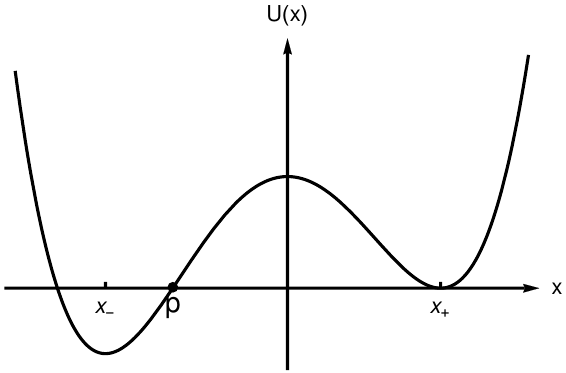
\includegraphics[scale = 0.3]{potencial.png}
        \caption{Potencial con un falso vacío}
        \label{fig:potencial}
    \end{figure}
    
    \item \textbf{Mecánica Clásica:} la partícula es estable en ambos mínimos.
    
    \item \textbf{Mecánica Cuántica:} si la partícula se encuentra en el mínimo del potencial con mayor energía ($x = x_+)$, va a decaer al de menor ($x = x_-$) por tunelamiento $\Rightarrow$ el potencial posee un falso vacío.
\end{itemize}
\end{frame}

\begin{frame}{Introducción}
\begin{itemize}
    \item Una partícula cuya función de onda se encuentra concentrada en la región del falso vacío no es un autoestado de energía; es un estado metaestable con energía compleja.
    %\item Para que haya decaimiento es necesario que la energía tenga una parte compleja.
    
    \item Probabilidad de que la partícula siga en la región del falso vacío luego de un tiempo $T$
    \begin{equation}
        P_{\mathrm{FV}}(T) = \int_{\mathrm{FV}} \dd{x} \qty| \psi (x, T) |^2
        \propto e^{-\Gamma T}
    \end{equation}
    donde
    \begin{equation}\label{eq:gammaE}
        \Gamma = -2 \mathrm{Im}\left(\frac{E_0}{\hbar}\right)
    \end{equation}
    es la tasa de decaimiento del estado metaestable. 
    
    %\begin{equation}
    %    \Gamma = \frac{1}{P_{\mathrm{FV}}(T)} \frac{d }{dt}P_{\mathrm{FV}}(T)
    %\end{equation}
\end{itemize}
\end{frame}

\begin{frame}{Aproximación WKB (Semiclásica)}
\begin{itemize}
    \item  La tasa de decaimiento es proporcional al coeficiente de transmisión a través de la barrera
    \begin{equation}
        \Gamma \propto T \propto e^{-B/\hbar}(1 + \mathcal{O}(\hbar))
    \end{equation}
    
    \begin{equation}\label{eq:decay}
        \Gamma = A e^{-B/\hbar} (1 + \mathcal{O}(\hbar))
    \end{equation}
    donde
    \begin{equation}\label{eq:BWKB}
        B = 2 \int_{x_+}^{x_0} dx \sqrt{2m \left(V(x) - E\right)}
    \end{equation}
    
    \item Cuando la partícula ($m = 1$) atraviesa la barrera en $x = x_0$, sale con energía cinética nula. Además en $V(x_0) = 0$ $\rightarrow E = 0$. En \eqref{eq:BWKB}
    \begin{equation}\label{eq:B}
        B = 2 \int_{x_+}^{x_0} dx \sqrt{2V(x)}
    \end{equation}
\end{itemize}

\end{frame}

\begin{frame}{Acción Euclideana}
\begin{itemize}
    \item Acción
    \begin{equation}
        S[x(t)] =  \int dt \left[ \frac{1}{2}\left(\frac{dx}{dt}\right)^2 - V(x) \right] 
    \end{equation}
    
    \item Rotación de Wick: $t = - i\tau \rightarrow$ Acción Euclideana
    \begin{equation}\label{eucliaction}
        S_E[x(\tau)] = \int d\tau \left[ \frac{1}{2}\left(\frac{dx}{d\tau}\right)^2 + V(x) \right] 
    \end{equation}
    
    \item Ecuación de movimiento
    \begin{equation}\label{eq:mov}
        \frac{d^2 x}{d\tau^2} = \frac{dV(x)}{dx} = -\frac{d(-V(x))}{dx}.
    \end{equation}
    Equivalente a una partícula moviéndose en el potencial $-V(x)$ en tiempo real. 
    
    \item Energía Euclideana
    \begin{equation}
        \mathcal{E} =  \frac{1}{2}\left(\frac{dx}{d\tau}\right)^2 - V(x)
    \end{equation}
\end{itemize}
\end{frame}

\begin{frame}{Bounce}
\begin{itemize}
    \item Solución a \eqref{eq:mov} con las siguientes condiciones
    \begin{subequations} \label{eq:CI}
    \begin{gather} \label{eq:eucliE}
        \mathcal{E}_B = 0 \\ \label{eq:CI1}
        \lim_{\tau \rightarrow \pm \infty} x_B = x_+ \quad x_B (0) = x_0
    \end{gather}
    \end{subequations}
    
    \begin{figure}
        \centering
        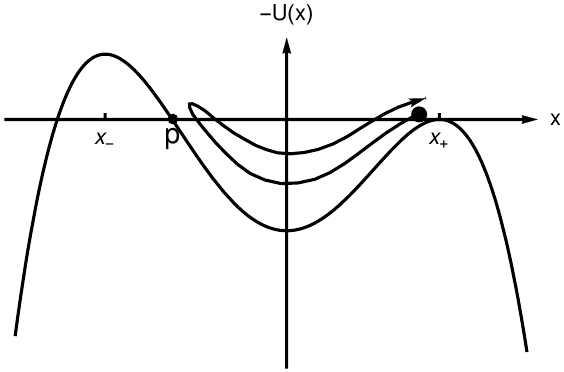
\includegraphics[scale = 0.22]{bounce.png}
        \caption{Bounce}
        \label{fig:bounce}
    \end{figure}
    \item En $\tau = 0$: $V(x_0) = 0$. De \eqref{eq:eucliE}
    \begin{equation}\label{eq:vel}
        \left. \frac{dx_B}{d\tau} \right|_{\tau = 0} = 0.
    \end{equation}
\end{itemize}
\end{frame}

\begin{frame}{Acción del Bounce}
\begin{itemize}
    \item Acción del bounce
    \begin{equation}\label{eq:bounce1}
        S_B =  \int_{-\infty}^{+\infty} d\tau \left[ \frac{1}{2}\left(\frac{dx_B}{d\tau}\right)^2 + V(x_B) \right] 
    \end{equation}
    
    \item De \eqref{eq:eucliE}
    \begin{equation}\label{eq:E0}
        \frac{1}{2}\left(\frac{dx_B}{d\tau}\right)^2 = V(x_B)
    \end{equation}
    
    \item Usando \eqref{eq:E0} en \eqref{eq:bounce1}
    \begin{equation}\label{eq:bounce2}
        S_B =   \int_{-\infty}^{+\infty} d\tau (2 V(x_B)) 
    \end{equation}
    
    \item El movimiento de la partícula es simétrico.
    \begin{equation}\label{eq:bounce3}
        S_B =  \int_{-\infty}^{0} d\tau (2 V(x_B)) + \int_{0}^{+\infty}  d\tau (2 V(x_B)) = 2 \int_{-\infty}^{0} d\tau (2 V(x_B))  
    \end{equation}
\end{itemize}
\end{frame}

\begin{frame}{Acción del Bounce}
\begin{itemize}
    \item Haciendo el cambio de variable $\tau \rightarrow x_B$. De \eqref{eq:E0}
    \begin{equation}\label{eq:dtau}
        d\tau = \frac{dx_B}{\sqrt{2V(x_B)}}
    \end{equation}
    
    \item Reemplazando \eqref{eq:dtau} en \eqref{eq:bounce3}
    \begin{equation}\label{eq:bounce4}
        S_B = 2 \int_{x_+}^{x_0} dx \sqrt{2 V(x)} 
    \end{equation}
    
    \item Comparando \eqref{eq:bounce4} con \eqref{eq:B}
    \begin{equation}
        \boxed{B = S_B}
    \end{equation}
\end{itemize}
\end{frame}

\begin{frame}{Integral de Camino Euclideana}
\begin{itemize}
    \item Amplitud de transición Euclideana (por conveniencia $\tau_f = T/2$ y $\tau_i = -T/2$)
    \begin{equation}\label{eq:amplitud}
        I = \bra{x_f, T/2} e^{-HT/\hbar} \ket{x_i, -T/2} = N \int \mathcal{D}[x] e^{-S_E/\hbar}
    \end{equation}
    
    \item Insertando un conjunto completo de autoestados de energía $\{ \ket{n} \}$ en \eqref{eq:amplitud}
    \begin{equation}\label{eq:Eeigen}
         I = \sum_n e^{-E_n T/\hbar} \phi^*_n(x_f, T/2) \phi_n(x_i, -T/2) 
    \end{equation}
    
    \item En el límite $T \rightarrow \infty$, el estado de menor energía domina la integral de camino en \eqref{eq:amplitud} 
    \begin{equation} \label{eq:Epi}
         \frac{E_0}{\hbar} = - \lim_{T \rightarrow \infty} \frac{\ln I}{T}
    \end{equation}
\end{itemize}
\end{frame}

\begin{frame}{Aproximación de Punto Estacionario}
\begin{itemize}
    \item El cálculo semiclásico de la integral de camino Euclideana en \eqref{eq:amplitud} requiere encontrar las soluciones a \eqref{eq:mov} que cumplan con las condiciones dadas. Estas corresponden a los puntos estacionarios (\emph{saddle point}) de la acción euclideana \eqref{eq:bounce1}.
    
    \item La integral de camino Euclideana se puede aproximar como la suma de las contribuciones de estos puntos.
    
    \item Equivalente a la aproximación WKB.
\end{itemize}
\end{frame}

\begin{frame}{Aproximación de Punto Estacionario}
\begin{itemize}
    \item La acción Euclideana es estacionaria para la trayectoria clásica
    \begin{equation}\label{eq:minimo}
        \frac{\delta S_E[x_{\textrm{cl}}]}{\delta x(\tau)} = 0.
    \end{equation}
    
    \item Expandiendo la acción alrededor de la trayectoria clásica
    \begin{equation} \label{eq:trayec}
        x(\tau) = x_{\textrm{cl}}(\tau) + \eta(\tau), \quad \eta(\tau_i) = \eta(\tau_f) = 0
    \end{equation}

    \begin{equation}
    \label{eq:Saprox}
    \begin{aligned} 
        S_{E}[x] &= S_{E}[x_{\textrm{cl}}(\tau) + \eta(\tau)] \\ 
            &= S_{E}[x_{\textrm{cl}}(\tau)] + \frac{1}{2} \iint  d\tau_1 d\tau_2  \eta(\tau_1) \frac{\delta^2 S_E[x_{\textrm{cl}}]}{\delta x_{\textrm{cl}}(\tau_1) \delta x(\tau_2)_{\textrm{cl}}} \eta(\tau_2) \\
            &\qquad + \mathcal{O}(\eta^3) \\ 
            &\approx S_E^{\textrm{cl}} + S_E^{(2)}[\eta(\tau)]
    \end{aligned}
    \end{equation}
\end{itemize}
\end{frame}

\begin{frame}{Aproximación de Punto Estacionario}
\begin{itemize}
    \item Usando \eqref{eq:Saprox} en \eqref{eq:amplitud}
    \begin{equation}\label{eq:Iaprox}
        I \approx N e^{-S_E^{\textrm{cl}}/\hbar} \int \mathcal{D}[x] e^{-S_E^{(2)}/\hbar}
    \end{equation}
    
    \item Para calcular $S_E^{(2)}$ partimos de \eqref{eq:bounce1} y tomamos las derivadas funcionales
    \begin{equation}\label{eq:2dev}
        \frac{\delta^2 S_E[x_{cl}]}{\delta x_{\textrm{cl}}(\tau_1) \delta x_{\textrm{cl}}(\tau_2)} = \left( -\frac{d}{d\tau_1} + V''(x_{\textrm{cl}}(\tau_1)) \right) \delta(\tau_1 - \tau_2)
    \end{equation}
    donde la prima denota la derivada respecto a $x(\tau)$.
    
    \item Reemplazando \eqref{eq:2dev} en \eqref{eq:Saprox} y aplicando el delta de Dirac
    \begin{equation}\label{eq:S2_1}
        S_E^{(2)} = \frac{1}{2} \int d\tau  \eta(\tau) \left( - \frac{d^2}{d\tau^2} + V''(x_{\textrm{cl}})\right) \eta(\tau)
    \end{equation}
\end{itemize}
\end{frame}

\begin{frame}{Aproximación de Punto Estacionario}
\begin{itemize}
    \item Introducimos un conjunto completo ortonormal de autofunciones del operador en \eqref{eq:S2_1}
    \begin{gather} \label{eq:eigen1}
        \left( - \frac{d^2}{d\tau^2} + V''(x_{\textrm{cl}})\right) \eta_\lambda(\tau) = \lambda \eta_\lambda(\tau) \\ \label{eq:eigen2}
        \int_{-T/2}^{T/2} d\tau  \eta_i(\tau) \eta_j(\tau) = \delta_{ij}
    \end{gather}
    
    \item Descomponemos $\eta(\tau)$ en función de estas autofunciones
    \begin{equation}\label{eq:eigen3}
        \eta(\tau) = \sum_\lambda a_\lambda \eta_\lambda (\tau) 
    \end{equation}

    \item Usando \eqref{eq:eigen1}, \eqref{eq:eigen2} y \eqref{eq:eigen3} en \eqref{eq:S2_1}
    \begin{equation}\label{eq:S2_3}
        S_E^{(2)} = \frac{1}{2} \sum_\lambda \lambda a_\lambda^2
    \end{equation}
\end{itemize}
\end{frame}

\begin{frame}{Aproximación de Punto Estacionario}
\begin{itemize}
    \item Haciendo el cambio de variable $x(\tau) \rightarrow \eta(\tau)$ con la medida
    \begin{equation}\label{medida}
        \mathcal{D}[\eta] = \prod_\lambda \frac{da_\lambda}{\sqrt{2\pi \hbar}}
    \end{equation}
    (se incluye el factor de $\sqrt{2\pi \hbar}$ por conveniencia).
    
    \item Reemplazando \eqref{eq:S2_3} y \eqref{medida} en \eqref{eq:Iaprox}, y desarrollando
    \begin{equation}
        I = N e^{-S_E^{\textrm{cl}}/\hbar} \prod_\lambda \lambda^{ -1/2}
    \end{equation}
    
    \item $\prod_\lambda \lambda^{ -1/2}$ es el determinante del operador en \eqref{eq:eigen1} por ser el producto de sus autovalores.
    
    \begin{equation}\label{Isaddle}
        \boxed{I = Ne^{-S_E^{\textrm{cl}} / \hbar} \left[ \det\left(-\frac{d^2}{d\tau^2} + V''(x_{\textrm{cl}}) \right)\right]^{-1/2}}
    \end{equation}
\end{itemize}
\end{frame}

\begin{frame}{Integral de Camino y Decaimiento del FV}
\begin{itemize}
    \item Existen algunos problemas con \eqref{Isaddle}
    \begin{itemize}
        \item Es real, por lo que la energía asociada no tiene parte imaginaria.
        
        \item Es válida solo cuando los autovalores son no negativos. 
    \end{itemize}
    
\item En el decaimiento del falso vacío $x_i = x_f = x_+$.

\item Existen 3 soluciones que cumplen con \eqref{eq:CI}: la solución constante $x(\tau) = x_+$, el bounce (de los cuales hay múltiples) y el shot. Solo se consideran las contribuciones de las dos primeras soluciones puesto que el shot da la energía del estado fundamental global y no la del falso vacio.
    
    \begin{figure}
        \centering
        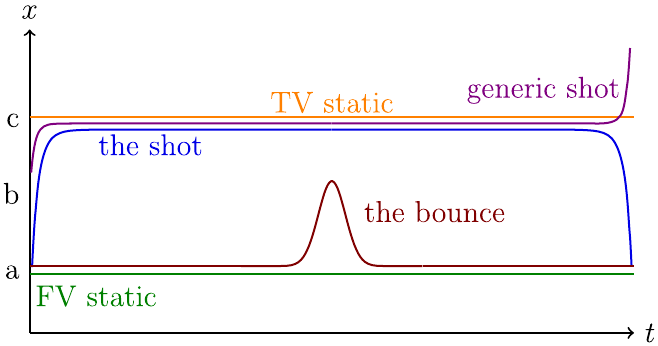
\includegraphics[scale = 0.23]{soluciones.png}
        \caption{Soluciones a las ecuaciones de movimiento Euclideana}
        \label{fig:my_label}
    \end{figure}
\end{itemize}
\end{frame}

\begin{frame}{Modo Cero}
\begin{itemize}
    \item Derivando \eqref{eq:mov} respecto a $\tau$ 
    \begin{equation}
        \left( - \frac{d^2}{d\tau^2} + V''(x_{\textrm{cl}})\right) \frac{dx_B}{d\tau} = 0
    \end{equation}
    $\rightarrow dx_B/d\tau$ es un modo cero del operador.
    
    \item Normalizando esta autofunción
    \begin{equation}
        x^{(0)}(\tau) = B^{-1/2}\frac{dx_B}{d\tau}
    \end{equation}
    
    \item La presencia de este modo cero se debe a la invariancia ante translaciones temporales del centro del bounce. Una variación de la forma $\delta \eta(\tau) \propto x^{(0)}(\tau)$ no cambia $S_E^{(2)}$.
\end{itemize}
\end{frame}

\begin{frame}{Modo Cero}
\begin{itemize}
    \item Si se integra el modo cero de la misma manera que el resto de autovalores no negativos, la integral en \eqref{eq:Iaprox} diverge. 
    
    \item Para integrar el modo cero introducimos la coordenada colectiva $\tau_0$ que corresponde al centro del bounce. Expandiendo la trayectoria usando esta nueva coordenada
    \begin{gather} \label{eq:expcentro}
        x(\tau) = x_B(\tau - \tau_0) + \eta (\tau - \tau_0) \\
        x(\tau + \tau_0) = x_B(\tau) + \eta (\tau) = x_B(\tau) + \sum_\lambda a_\lambda \eta_\lambda (\tau)
    \end{gather}
    
    \item Separando $a_0$ en \eqref{eq:eigen3} y usando \eqref{eq:expcentro}
    \begin{equation} \label{eq:a02}
        a_0 (\tau_0) = \int_{-T/2}^{T/2} d\tau x(\tau + \tau_0) x_0(\tau) 
    \end{equation}
\end{itemize}
\end{frame}

\begin{frame}{Modo Cero}
\begin{itemize}
    \item Derivando \eqref{eq:a02} respecto a $\tau_0$ 
    \begin{align}
        \frac{da_0}{d\tau_0} &= \int_{-T/2}^{T/2} d\tau \frac{dx(\tau + \tau_0)}{d\tau_0}  x_0(\tau) =  \int_{-T/2}^{T/2} d\tau \frac{dx(\tau + \tau_0)}{d\tau}  x_0(\tau) \\
            &= \int_{-T/2}^{T/2} d\tau
            \left( \frac{dx_B(\tau)}{d\tau_0} +  \sum_\lambda a_\lambda  \frac{d\eta_\lambda(\tau)}{d\tau} \right) x_0(\tau) \\
            &\approx \int_{-T/2}^{T/2} d\tau
            \frac{dx_B(\tau)}{d\tau_0} x^{(0)}(\tau) \\
            &= B^{1/2} \int_{-T/2}^{T/2} d\tau x_0^2(\tau) \\
            &= B^{1/2} 
    \end{align}
    ($x_0(\tau)$ esta normalizado)
\end{itemize}
\end{frame}

\begin{frame}{Modo Cero}
\begin{itemize}
    \item Haciendo el cambio de variable $a_0 \rightarrow t_0$ en \eqref{medida} y desarrollando
    \begin{equation} \label{eq:I0}
        I_1 =\left( \frac{B}{2\pi \hbar} \right)^{1/2} \left[ \textrm{det}' \left(-\frac{d^2}{d\tau^2} + V''(x_{\textrm{cl}}) \right)\right]^{-1/2} T e^{-B/\hbar}
    \end{equation}
    donde $\textrm{det}'$ indica que no se considera el modo cero en la determinante (se elige la normalización de tal manera que $N = 1$ en \eqref{eq:Iaprox}). El subíndice indica que esta contribución corresponde a la de un único bounce. 
\end{itemize}
\end{frame}

\begin{frame}{Modo Negativo}
\begin{itemize}
    \item De \eqref{eq:vel} notamos que $x_0(\tau)$ tiene un nodo. Sabemos (por ejemplo) de la ecuación de Schr\"{o}dinger que la autofunción correspondiente a la energía fundamental no tiene nodos. Eso implica que el operador en \eqref{Isaddle} posee una autofunción con autovalor negativo $\rightarrow$ modo negativo.
    
    \item Al igual que el modo cero, el modo negativo hace que la integral en \eqref{eq:Iaprox} diverga. En este caso para realizar la integración se introduce un parámetro en la acción y se hace la continuación analítica del contorno de integración al plano complejo.
    
    \item Esto da como resultado un factor de $i/2$ en \eqref{eq:I0}
    \begin{equation} \label{eq:negativo}
        I_1 = \frac{i}{2} \left( \frac{B}{2\pi \hbar} \right)^{1/2}  \left[ \textrm{det}' \left(-\frac{d^2}{d\tau^2} + V''(x_{\textrm{cl}}) \right)\right]^{-1/2} T e^{-B/\hbar}
    \end{equation}
    donde $\textrm{det}'$ indica ahora que solo se consideran los autovalores mayores que cero. 
\end{itemize}
\end{frame}

\begin{frame}{Contribución de Múltiples Bounces}
\begin{itemize}
    \item En \eqref{eq:amplitud} se debe considerar la contribución de un número arbitrario de bounces. 
    
    \item Definiendo 
    \begin{equation}
        K = \frac{1}{2} \left(\frac{B}{2\pi\hbar}\right)^{1/2} \left[ \frac{\textrm{det}' \left(-\frac{d^2}{d\tau^2} + V''(x_{\textrm{cl}}) \right)}{\det \left(-\frac{d^2}{d\tau^2} + \omega^2 \right)}\right]^{-1/2}
    \end{equation}
    donde $\omega^2 = V''(x_+)$podemos escribir la contribución de un número arbitrario de bounces como 
    \begin{equation}
        I_n = \frac{1}{n!} \left(iKTe^{-B}\right)^n I_0
    \end{equation}
    donde $I_0$ es la contribución de la solución constante y se incluye factor de $n!$ debido a que los bounces son indistinguibles.
\end{itemize}
\end{frame}

\begin{frame}{Contribución de Múltiples Bounces}
\begin{itemize}
    \item Sumando todas las contribuciones
    \begin{equation}\label{eq:Itotal}
        I = \sum_{n = 0}^{\infty} I_n = I_0 \exp{\left(iKTe^{-B/\hbar}\right)}
    \end{equation}
    
    \item Finalmente, reeemplazando \eqref{eq:Itotal} en \eqref{eq:Epi} y luego en \eqref{eq:gammaE} ($I_0$ no posee parte imaginaria)
    \begin{equation}
        \boxed{\Gamma = \left(\frac{B}{2\pi\hbar}\right)^{1/2}  \left[ \frac{\textrm{det}' \left(-\frac{d^2}{d\tau^2} + V''(x_{\textrm{cl}}) \right)}{\det \left(-\frac{d^2}{d\tau^2} + \omega^2 \right)}\right]^{-1/2}e^{-B/\hbar}\left( 1 + \mathcal{O}(\hbar)\right)}.
\end{equation}
\end{itemize}
\end{frame}
\end{document}